%----------------------------------------
\subsection{Stencil codes}
\label{sect:stencil}
%----------------------------------------
To numerically solve a set of PDEs, iterative methods (finite difference, finite volume, finite element methods etc.) are frequently used to approximate the solution through a discretized (step by step) phenomena. Thus, the continuous time and space domains are discretized so that a set of numerical computations are iteratively (time discretization) applied onto a mesh (space discretization). In other words, in a mesh-based numerical simulation, the PDEs are transformed to a set of numerical computations applied at each time step on elements of the discretized space domain (the mesh). Among those numerical computations is found a set of numerical schemes, also called \textit{stencil computations}~\cite{spaaTangCKLL11}. To ease programming of stencil computations, and because of the relative regularity of such a computation, many solutions (languages or libraries) propose an easy way to describe the stencil code, while producing transparently an optimized and parallelized stencil code. For example, Liszt~\cite{DeVito2011LDS} and OP2~\cite{Giles2011} are domain specific languages to define a stencil code on unstructured meshes, while Pochoir~\cite{spaaTangCKLL11} and PATUS~\cite{citeulike12258902} address structured meshes, respectively proposing an optimized cache tiling technique, and a separation of concerns by separating parallelization strategy from the computation description.

Let introduce some concepts used in this paper. First, a stencil code is based on a \emph{mesh} which is the discretization of the physical real domain. A mesh is a connected undirected graph without bridges (an edge is a bridge if its removal results in two disconnected graphs), where nodes and edges are linked to form cells (closure). For example, a structured mesh is illustrated in Figure~\ref{fig:ex}, each cell contains four nodes and four edges. Second, \emph{mesh domains} are subset elements of the mesh, such as the center of cells, edges or nodes, for example. In Figure~\ref{fig:ex} two mesh domains are used, the center of the cells (in red) and the edge on the horizontal axe (in blue on the left and right of each cell). A \emph{data} is a quantity to simulate or a temporary data to perform computations. A data is mapped onto a given mesh domain. For example, in Figure~\ref{fig:ex}, data $A$ and $B$ are mapped onto the center of cells, while $C$ is mapped onto the edges.

\begin{figure}[!h]\begin{center}
  \resizebox{7cm}{!}{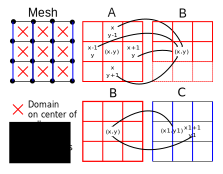
\includegraphics{./images/stencil.pdf}}
  \caption{Examples of a stencil computations}
  \label{fig:ex}
\end{center}\end{figure}

The first stencil computation in Figure~\ref{fig:ex} computes $B$ using $A$, while the second one computes $B$ using $C$. Thus, a stencil computation is defined by a set of input data (in those examples only one input data), and a single output data, the result. The \emph{computation domain} is a subset of elements to compute on the output data. In other words a computation domain is a subset of a mesh domain. For example, in the first stencil, the computation of $B$ is performed on plain elements, while dotted elements are not computed. On the other hand, on the second computation, the computation domain of $B$ is exactly equal to the cell mesh domain. The computation domain represents the set of elements on which the computation is performed, in other words, the space loop.

Finally, a stencil computation is composed of a \emph{numerical expression} which indicates how to compute an element of the computation domain (on the output data), using elements of the set of input data. The numerical expression of a stencil computation has the particularity to use not only the element to compute but also a \emph{neighborhood} of this element, also called a \emph{stencil shape}. For example, the stencil shape of the first computation in Figure~\ref{fig:ex} contains direct neighbors on the right, left, top and bottom. Sometimes, the neighborhood shape can also access a different mesh domain, as for example in the second computation example. Actually, in this computation, the neighborhood contains edges on the left and on the right of the cell. As a result, we could imagine for example that the numerical expression of the first example is
\begin{equation*} 
B(x,y) = A(x+1,y)+A(x-1,y)+A(x,y+1)+A(x,y-1),
\end{equation*}
and that the numerical expression of the second example is
\begin{equation*} 
B(x,y) = B(x,y)+C(x1,y1)+C(x1+1,y1).
\end{equation*}

To conclude this section, we define a stencil computation $s$ as the quintuplet
\begin{equation} 
s(R,w,exp,\mathcal{N},d_c),
\label{eq:st}
\end{equation}
where $R$ is the set of input data, $w$ the output data, $exp$ the numerical expression of the stencil computation, which is applied on the computation domain $d_c$, using a stencil shape $\mathcal{N}$.

%----------------------------------------
\subsection{Multi-stencil programs}
\label{sect:multistencil}
%----------------------------------------
While stencil computations are well defined and a lot studied in the literrature, it is not the case for real case numerical simulations. In this paper, we define what we call a \emph{multi-stencil program}, which actually is a general numerical simulation. 

A real case numerical simulation is most of the time not composed of a single stencil computation, but of a set of stencil computations, with one or more stencil shapes (neighboorhood), and onto one or more data. Moreover, a numerical simulation also performs additionnal auxiliary computations which do not involve neighborhood, called local computations. This paper targets this general case of numerical simulations that we call \emph{multi-stencil programs}. The work presented produces a general parallelization structure of the overall simulation, while most stencil solutions produce optimized codes for a single stencil code. As it will be detailed in the related work, this work is complementary to the optimization and parallelization of a single stencil computation.

An auxiliary computation is almost the same than a stencil computation, however its numerical expression does not involve a neighborhood, which makes this kind of computation purely local. A local computation $l$ is defined as the quadruplet
\begin{equation} 
l(R,w,exp,d_c),
\label{eq:loc}
\end{equation}
where $R$ is the set of input data, $w$ the output data, $exp$ the numerical expression of the stencil computation, which is applied on the computation domain $d_c$.

A multi-stencil program in this work is defined as a sextuplet
\begin{equation} 
\mathcal{MSP}(T,\mathcal{M},\mathcal{D}_m,\mathcal{D}_c,\Delta,\Gamma),
\label{eq:msp}
\end{equation}
where $T$ is the set of time iteration to run the simulation, $\mathcal{M}$ is the mesh of the simulation, $\mathcal{D}_m$ is the set of mesh domains, $\mathcal{D}_c$ is the set of computation domains used into computations, $\Delta$ is the set of data, each one mapped onto a mesh domain, and finally $\Gamma$ is the set of computations. The set of computations $\Gamma$ is composed of an ordered list of stencil and local computations. One can notice that this work is limited to a single type of mesh in a given simulation.

%----------------------------------------
\subsection{Parallelization techniques}
\label{sect:parallel}
%----------------------------------------
Three classical parallelization techniques are used in this paper and are described in this section, the data parallelism, the task parallelism, and the hybrid data and task parallelism. Those parallelization techniques are independent from the actual parallel hardware used.

\paragraph{Data parallelism} The idea of this parallelization technique is to split, or partition, data on which computations are applied among available processors (or cores). Each processor then applies the same progam or instruction onto its subpart of data. Moreover, if a neighborhood information is needed from another processor communications or synchronizations are performed. 

In the domain of numerical simulations, this technique is most of the time called a domain decomposition. This parallelization technique produce efficient programs up to thousands processors or cores, but on certain conditions. First, each subpart of data has to be big enough to overlap communication time. Second, the partitioning of data has to be balanced among processors. Thus, if this parallelization technique is clearly adequate to structured meshes, easy to balance, it is not for unstructured meshes or irregular structures where the amount of work is not heterogenous.

\paragraph{Task parallelism} Another well known parallelization technique is to identify in a program the different tasks and which one are independant and can be launched concurrently. Most of the time, such a prallelization technique create a dependency directed acyclic graph (dependency dag) from a set of ordered tasks. Dependencies are found from read/write information for each task. Actually, if a task $i$ write a data $a$ and if a task $j$ read $a$, then $i$ has to be finished before $j$ is performed. From a dependency graph two different solutions are available. First, a static schedule of tasks is built, which could be a good solution if the tasks are regular, or use a dynamic scheduler to dynamically decide at runtime which task is executed on which processor.

\paragraph{Hybrid parallelism} Finally, it is also possible to combine both those parallelization techniques to get what is called an hybrid parallelization. The interest of an hybrid parallelization is to bring another source of parallelism if limits of a given technique are reach.

%----------------------------------------
\subsection{Component models}
%----------------------------------------
Component model is an interesting domain of software engineering~\cite{Szyperski:2002:CSB:515228}, where functionnalities of an application are dispatched in different entities called components. Component models improves code re-use by a separation of concerns, scalability and maintainability of applications~\cite{Szyperski:2002:CSB:515228,bigot:inria-00388508}. In addition to this, recent work on component models have shown a simultaneous answer to performance, maintainability and portability of applications~\cite{l2c}, which makes this domain an interesting solution to bring maintainability and portability in HPC programming.
Many component models exist, each of them with its own specification and singularity, like CCM~\cite{corba:omg06} (CORBA Component Model), GCM~\cite{Baude} (Grid Component Model) or CCA~\cite{Armstrong:1999:TCC:822084.823232} (Common Component Architecture), for example. 

In the rest of this paper will be used concepts of the component model $L^2C$~\cite{l2c}. $L^2C$ is a minimalist HPC-oriented component model where a component extends the concept of class by specifying in its interfaces not only the services it offers, but also all its possible interactions with outer world. As a result, each component is an independant entity composed of a set of services its provides, and a set of services it requires (and uses). 
A \emph{port} in $L^2C$ is an entity embbedded in the component which makes possible an \emph{assembly} of components. An assembly of components is a way to actually connect components together and to produce a complete application, as a set of components and their interactions. A provided service inside a component is associated to a \emph{provide} port, while a required service is associated to a \emph{use} port. It is also possible to group more than one required service into a single port, as a list, called a \emph{use-multiple} port. As illustrated in Figures~\ref{fig:ports}, a provide port will be represented by a white circle on the left of the component, a use port by a black circle and a use-multiple port by a black circle with a white $m$ in it, both on the right of the component.

\begin{figure}[h!]
\begin{center}
\begin{tikzpicture}[shorten >=1pt, node distance=2cm, on grid, auto]
   \node[component] (C) at (0,0) {$Comp_0$};
   \node[provide] (p) at (-1.5,0) {};
   \node[use] (u) at (1.5,0) {};
   \node[provide,right=1.5cm of u] (p1) {};
   \node[component,right=1.5cm of p1] (C1) {$Comp_1$};
   \node[use,right=1.5cm of C1] (um) {$m$};
 
  \path[-]
    (p) edge node {} (C)
    (C.east) edge node {} (u)
    (C1)	edge node {} (um)
    (p1) edge node {} (C1);
\end{tikzpicture}
\caption{Two components, one with a provide, use and use-multiple ports, the second with a single provide port}
\label{fig:ports}
\end{center}
\end{figure}

In the rest of this paper, when a required service of a \emph{use} (or \emph{use-multiple}) port is filled and linked to a \emph{provide} port in the comonent assembly, only the use port stay visible, as illustrated in Figure~\ref{fig:assembly}. As the use port is on the right of its component, and the provide port on the left, in a component assembly the component on the left uses the provide port of the component on the right.

\begin{figure}[h!]
\begin{center}
\begin{tikzpicture}[shorten >=1pt, node distance=2cm, on grid, auto]
   \node[component] (C) at (0,0) {$Comp_0$};
   \node[provide] (p) at (-1.5,0) {};
   \node[use] (u) at (1.5,0) {};
   \node[component,right=1.5 of u] (C1) {$Comp_1$};
   \node[use,right=1.5 of C1] (um) {$m$};
 
  \path[-]
    (p) edge node {} (C)
    (C) edge node {} (u)
    (C1)	edge node {} (um)
    (u) edge node {} (C1);
\end{tikzpicture}
\caption{Component assembly of Figure~\ref{fig:ports}}
\label{fig:assembly}
\end{center}
\end{figure}

With its minimal set of ports, $L^2C$ is a light component model which does not introduce overheads at runtime, and which results in a HPC-oriented component model. Another HPC-oriented component model is CCA~\cite{Armstrong:1999:TCC:822084.823232}, however the main difference between those component models is the way a distribution of component on distributed architectures is managed. Actually, in CCA distant components (on different processors or machines) have to be managed manually inside components using MPI~\cite{Graham2009MSE} (Message Passing Interfaces), while $L^2C$ proposes a specific MPI port to link distant components and ease their communications. Moreover, by exposing MPI connections, $L^2C$ also exposes the parallel structure of a program inside the assembly, which increase separation of concerns and code reuse for parallel applications.

